\documentclass{beamer}
\usetheme{Madrid}
\usepackage[T1]{fontenc}
\usepackage{mathpazo}
\usepackage{graphicx}
\usepackage{booktabs}
\usepackage{tikz}
\usetikzlibrary{positioning,arrows.meta,shapes.geometric,fit,backgrounds,calc}
\definecolor{cetnavy}{RGB}{10,26,63}
\definecolor{cetlight}{RGB}{225,231,242}
\setbeamercolor{structure}{fg=cetnavy}
\setbeamercolor{frametitle}{bg=cetnavy,fg=white}
\setbeamercolor{title}{bg=cetnavy,fg=white}
\setbeamertemplate{navigation symbols}{}
% =====================================================================
%  EDIT YOUR DETAILS HERE — this ONE file feeds every abstract & deck.
%  (Change a value, recompile; all 36 documents update.)
% =====================================================================
\newcommand{\seminarName}{Aflah Muhammed P}      % <-- your full name (guessed from your email; please verify)
\newcommand{\seminarRoll}{TVE00CS000}            % <-- your university register/roll number
\newcommand{\seminarClassRoll}{00}               % <-- your class roll no (the short one)
\newcommand{\seminarGuide}{Prof.\ <Guide Name>}  % <-- your guide
\newcommand{\seminarDept}{Department of Computer Science and Engineering}
\newcommand{\seminarCollege}{College of Engineering Trivandrum}
\newcommand{\seminarShortCollege}{CET}           % shown in the slide footer, e.g. "Aflah Muhammed P (CET)"
\newcommand{\seminarShortTitle}{B.Tech Seminar}  % middle of the slide footer
\newcommand{\seminarDate}{July 31, 2026}
% ---------------------------------------------------------------------
% Optional: put a logo image named  cet_logo.png  in this folder and it
% will appear on every title slide automatically. If absent, it is skipped.
% =====================================================================

\title[\seminarShortTitle]{DeepRAG: Teaching Language Models When to Retrieve}
\author[\seminarName\ (\seminarShortCollege)]{\seminarName \\ \seminarRoll \\ Roll No: \seminarClassRoll \\ Guide: \seminarGuide}
\institute[\seminarShortCollege]{\seminarDept \\ \seminarCollege}
\date{\seminarDate}
\titlegraphic{\IfFileExists{cet_logo.png}{\includegraphics[height=1.1cm]{cet_logo.png}}{}}
\begin{document}
\begin{frame}\titlepage\end{frame}
\begin{frame}{Table of Contents}\tableofcontents\end{frame}
\section{Introduction}
\begin{frame}{Grounding LLMs with Retrieval}
\begin{itemize}
\item LLMs reason fluently but hallucinate facts.
\item RAG grounds answers in external documents.
\item Naive RAG retrieves for every query.
\item This adds noise, latency, and cost.
\end{itemize}
\end{frame}

\begin{frame}{The Core Question}
\begin{itemize}
\item When should a model actually retrieve?
\item Some sub-questions need external evidence.
\item Others sit inside parametric memory.
\item DeepRAG learns this choice step by step.
\end{itemize}
\end{frame}

\section{Literature Survey}
\begin{frame}{Prior Retrieval Strategies}
\textbf{\textit{From static to adaptive retrieval}}
\begin{itemize}
\item Classic RAG: fixed retrieve-then-read pipelines.
\item Adaptive: Self-RAG, FLARE use confidence triggers.
\item Iterative: IRCoT, Iter-RetGen retrieve repeatedly.
\item Heuristic triggers lack end-to-end training.
\item Reasoning-focused LLMs ignore retrieval timing.
\end{itemize}
\end{frame}

\section{Motivation}
\begin{frame}{Why Smarter Retrieval Matters}
\begin{itemize}
\item Retrieving every step injects irrelevant passages.
\item Redundant retrieval raises latency and cost.
\item Weak decomposition hurts multi-hop questions.
\item Models poorly sense their knowledge boundary.
\item Need learned, adaptive retrieval decisions.
\end{itemize}
\end{frame}

\section{Problem Statement}
\begin{frame}{Problem Statement}
\begin{itemize}
\item Decide, per sub-question, whether to retrieve.
\item Balance answer accuracy against retrieval cost.
\item Suppress noise from unnecessary documents.
\item Avoid brittle hand-crafted heuristics.
\end{itemize}
\end{frame}

\section{Objectives}
\begin{frame}{Objectives and Contributions}
\begin{itemize}
\item Cast retrieval-augmented reasoning as an MDP.
\item Decompose queries into atomic sub-questions.
\item Learn when parametric knowledge suffices.
\item Calibrate awareness of knowledge boundaries.
\item Improve accuracy and efficiency jointly.
\end{itemize}
\end{frame}

\section{Methodology Overview}
\begin{frame}{The Retrieval Narrative}
\begin{itemize}
\item Answer built as an iterative narrative.
\item Each step yields one atomic sub-query.
\item Termination action: decompose further or stop.
\item Atomic decision: retrieve or use memory.
\end{itemize}
\end{frame}

\begin{frame}{Per-Step Retrieval Decision}
\begin{center}
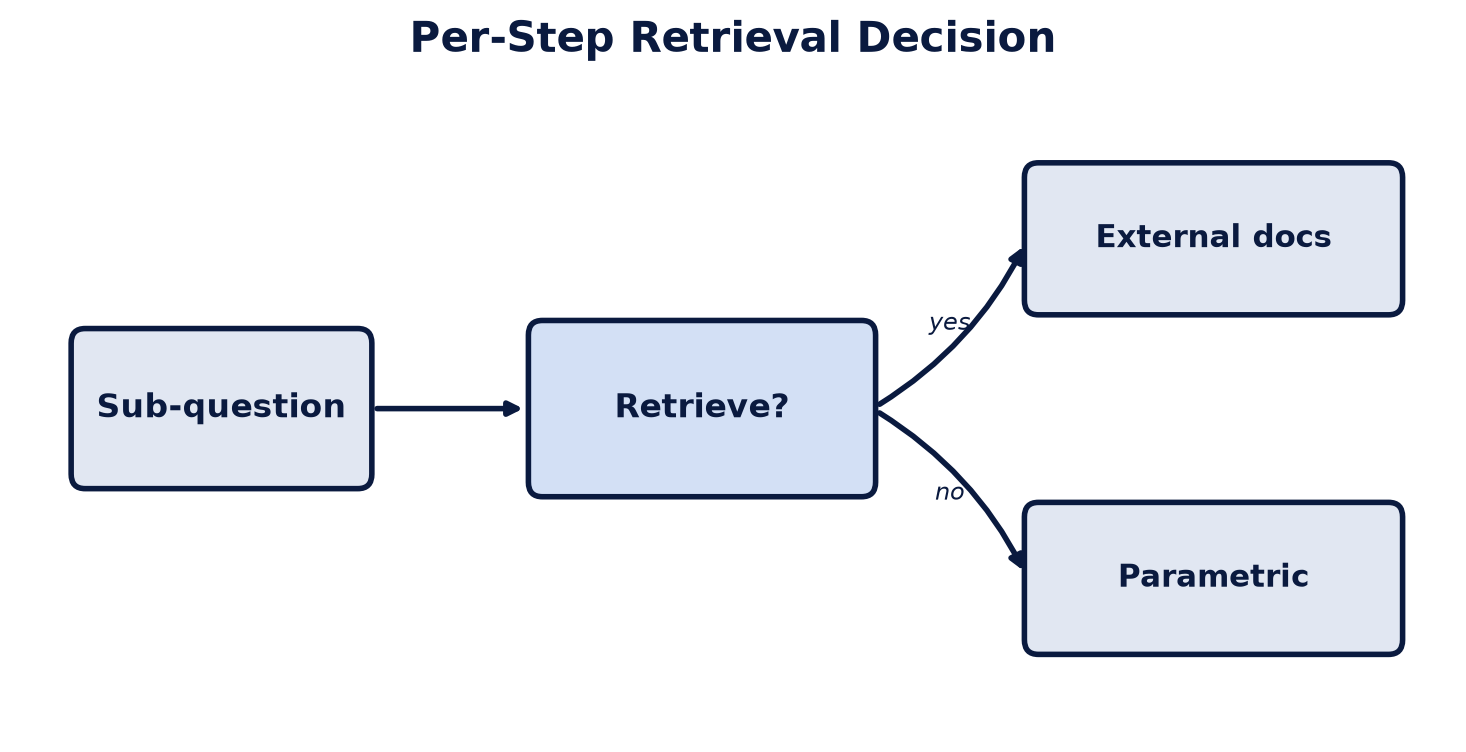
\includegraphics[width=0.9\textwidth,height=0.62\textheight,keepaspectratio]{images/deeprag_1.png}
\end{center}
\end{frame}

\section{System Architecture}
\begin{frame}{Three-Stage Training Framework}
\begin{itemize}
\item Stage 1: binary tree search synthesizes paths.
\item Stage 2: imitation learning on optimal narratives.
\item Stage 3: chain of calibration refines boundaries.
\item Output: an adaptive retrieval-aware model.
\end{itemize}
\end{frame}

\begin{frame}{Training Pipeline}
\begin{center}
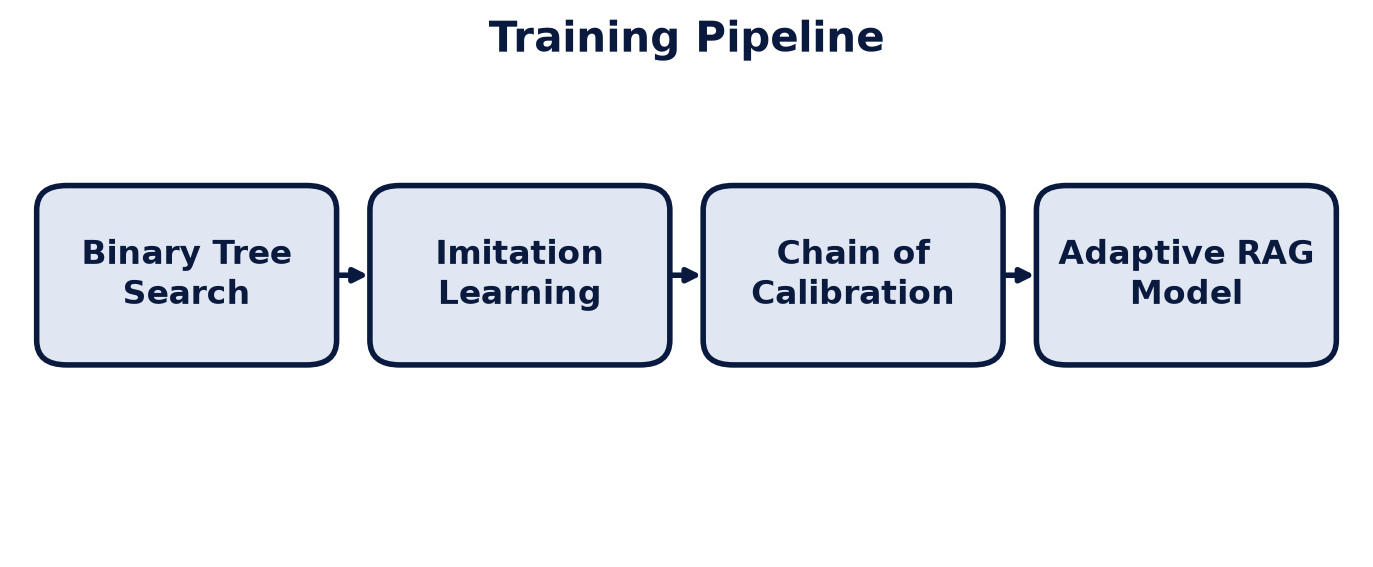
\includegraphics[width=0.9\textwidth,height=0.62\textheight,keepaspectratio]{images/deeprag_2.png}
\end{center}
\end{frame}

\section{Data Collection}
\begin{frame}{Datasets and Setup}
\begin{itemize}
\item Trained on HotpotQA and 2WikiMultihopQA.
\item 4{,}000 imitation samples per dataset.
\item 1{,}000 calibration samples per dataset.
\item Tested in- and out-of-distribution.
\item Extra benchmarks: PopQA, CAG, WebQuestions.
\end{itemize}
\end{frame}

\section{Model Development}
\begin{frame}{Learning When to Retrieve}
\begin{itemize}
\item Tree search explores retrieve vs.\ no-retrieve branches.
\item Prefers correct paths with fewest retrievals.
\item Imitation learning on these optimal trajectories.
\item Calibration via preference optimization.
\item Teaches the model its own boundary.
\end{itemize}
\end{frame}

\section{Results}
\begin{frame}{Main Findings}
\begin{itemize}
\item About 21.99\% average accuracy gain.
\item Fewer retrievals than always-retrieve RAG.
\item Gains on Llama-3-8B and Qwen-2.5-7B.
\item Strong out-of-distribution generalization.
\end{itemize}
\end{frame}

\begin{frame}{Accuracy vs.\ Baseline}
\begin{center}
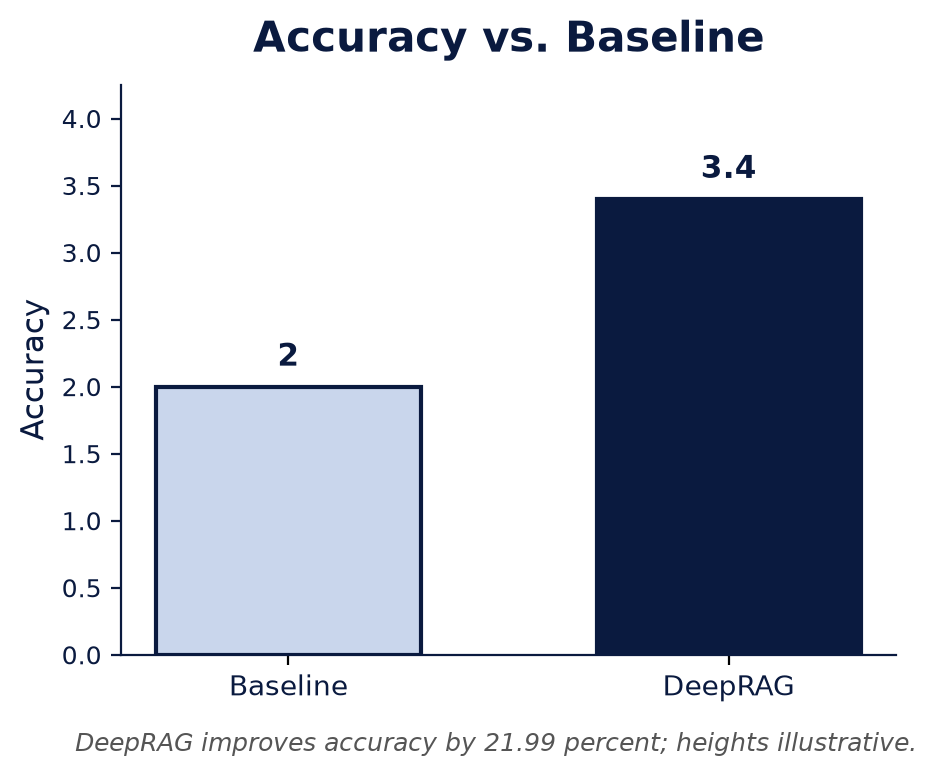
\includegraphics[width=0.9\textwidth,height=0.62\textheight,keepaspectratio]{images/deeprag_3.png}
\end{center}
\begin{center}
\footnotesize Higher accuracy with fewer retrievals (illustrative).
\end{center}
\end{frame}

\section{Discussions}
\begin{frame}{Why It Works}
\begin{itemize}
\item Selective retrieval cuts distracting passages.
\item Decomposition aligns retrieval with reasoning.
\item Calibration links parametric knowledge to decisions.
\item Accuracy and efficiency improve together.
\end{itemize}
\end{frame}

\section{Challenges}
\begin{frame}{Limitations}
\begin{itemize}
\item Binary tree search is compute-intensive offline.
\item Depends on retriever and corpus quality.
\item Knowledge-boundary estimates stay imperfect.
\item Evaluated mainly on factual QA.
\end{itemize}
\end{frame}

\section{Future Work}
\begin{frame}{Future Directions}
\begin{itemize}
\item Extend beyond QA to complex reasoning.
\item Cheaper alternatives to tree-search synthesis.
\item Tighter knowledge-boundary calibration.
\item Integrate stronger adaptive retrievers.
\end{itemize}
\end{frame}

\section{Conclusion}
\begin{frame}{Conclusion}
\begin{itemize}
\item Retrieval timing is a learnable decision.
\item MDP framing enables step-by-step retrieval.
\item DeepRAG lifts accuracy and efficiency.
\item A path toward trustworthy, efficient RAG.
\end{itemize}
\end{frame}

\section{References}
\begin{frame}{References}
\footnotesize
\begin{itemize}
\item X. Guan, J. Zeng, F. Meng, et al., ``DeepRAG: Thinking to Retrieve Step by Step for Large Language Models,'' arXiv:2502.01142, 2025.
\item A. Asai, Z. Wu, Y. Wang, A. Sil, and H. Hajishirzi, ``Self-RAG: Learning to Retrieve, Generate, and Critique through Self-Reflection,'' in Proc. ICLR, 2024.
\item Z. Jiang, F. F. Xu, L. Gao, et al., ``Active Retrieval Augmented Generation,'' in Proc. EMNLP, 2023.
\end{itemize}
\end{frame}
\begin{frame}\vfill\centering{\Huge Thank You}\vfill\end{frame}
\end{document}
